% 5-minute pitch draft (Exercise 4); the final version goes to Google Slides.
% Every number comes from the Python scripts in the repo root; figures are in ../figures/.
% Build: latexmk -pdf presentation.tex   (build files go to build/, see latexmkrc)
\documentclass[aspectratio=169,11pt]{beamer}
\usetheme{default}
\setbeamertemplate{navigation symbols}{}
\setbeamertemplate{footline}{\hfill\scriptsize\color{gray}\insertframenumber\hspace{1.2em}\vspace{0.6em}}
\definecolor{ink}{HTML}{0B0B0B}
\definecolor{ink2}{HTML}{52514E}
\definecolor{muted}{HTML}{898781}
\definecolor{good}{HTML}{0CA30C}
\definecolor{warn}{HTML}{B07A00}
\definecolor{bad}{HTML}{D03B3B}
\setbeamercolor{frametitle}{fg=ink}
\setbeamercolor{title}{fg=ink}
\setbeamercolor{subtitle}{fg=ink2}
\setbeamercolor{normal text}{fg=ink}
\setbeamercolor{structure}{fg=ink2}
\setbeamerfont{frametitle}{series=\bfseries,size=\Large}
\setbeamertemplate{itemize items}{\textbullet}
\usepackage{booktabs}
\usepackage{tabularx}
\graphicspath{{../figures/}}
\newcommand{\smallnote}[1]{{\scriptsize\color{muted}#1}}

\title{Two independent eyes on every direction}
\subtitle{Sensor modality comparison: compare and design a city + highway car}
\author{Team: \textit{names TBD}}
\date{3DSSF -- Kozma -- Exercise 4}

\begin{document}

\begin{frame}
  \titlepage
\end{frame}

% ---------------------------------------------------------------
\begin{frame}{1. What must the car see, and how far?}
  \begin{columns}[c]
    \column{0.46\textwidth}
    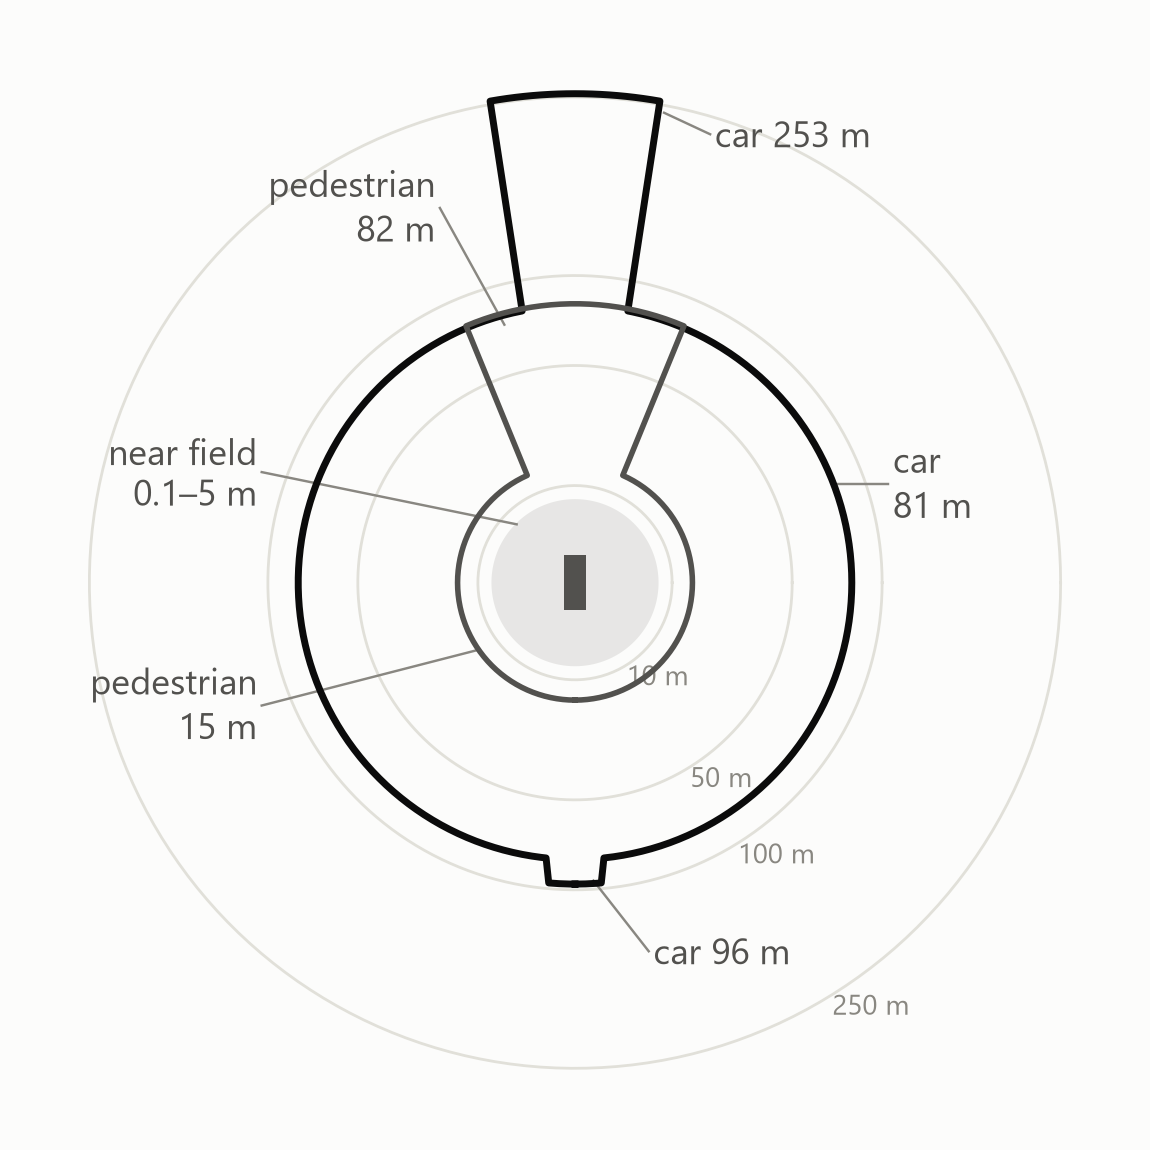
\includegraphics[width=\textwidth]{requirements.png}
    \column{0.52\textwidth}
    \small
    \renewcommand{\arraystretch}{1.15}
    \begin{tabularx}{\textwidth}{@{}lXr@{}}
      \toprule
      where & scenario & range \\
      \midrule
      ahead & stop for a car from 130\,km/h & \textbf{253\,m} \\
      ahead & stop for a pedestrian from 70\,km/h & \textbf{82\,m} \\
      sides & pull out before cross traffic (60\,km/h) & \textbf{81\,m} \\
      behind & lane change, car closing at 60\,km/h & \textbf{96\,m} \\
      around & jogger during a 4.9\,s turn & \textbf{15\,m} \\
      around & kerbs, a child next to the car & \textbf{0.1--5\,m} \\
      \bottomrule
    \end{tabularx}

    \vspace{0.3em}
    \smallnote{stopping distance $v\cdot 1\,\mathrm{s} + v^2/(2\cdot 3\,\mathrm{m/s^2})$: plan to stop without emergency braking}

    \vspace{0.8em}
    \textbf{Design rule:} on every bearing, at least \textbf{two independent modalities}
    (camera, lidar, radar, thermal) reach the required range
    -- so one can fail or be fooled.
  \end{columns}
\end{frame}

% ---------------------------------------------------------------
\begin{frame}{2. Compare: no modality wins every axis in every condition}
  \centering
  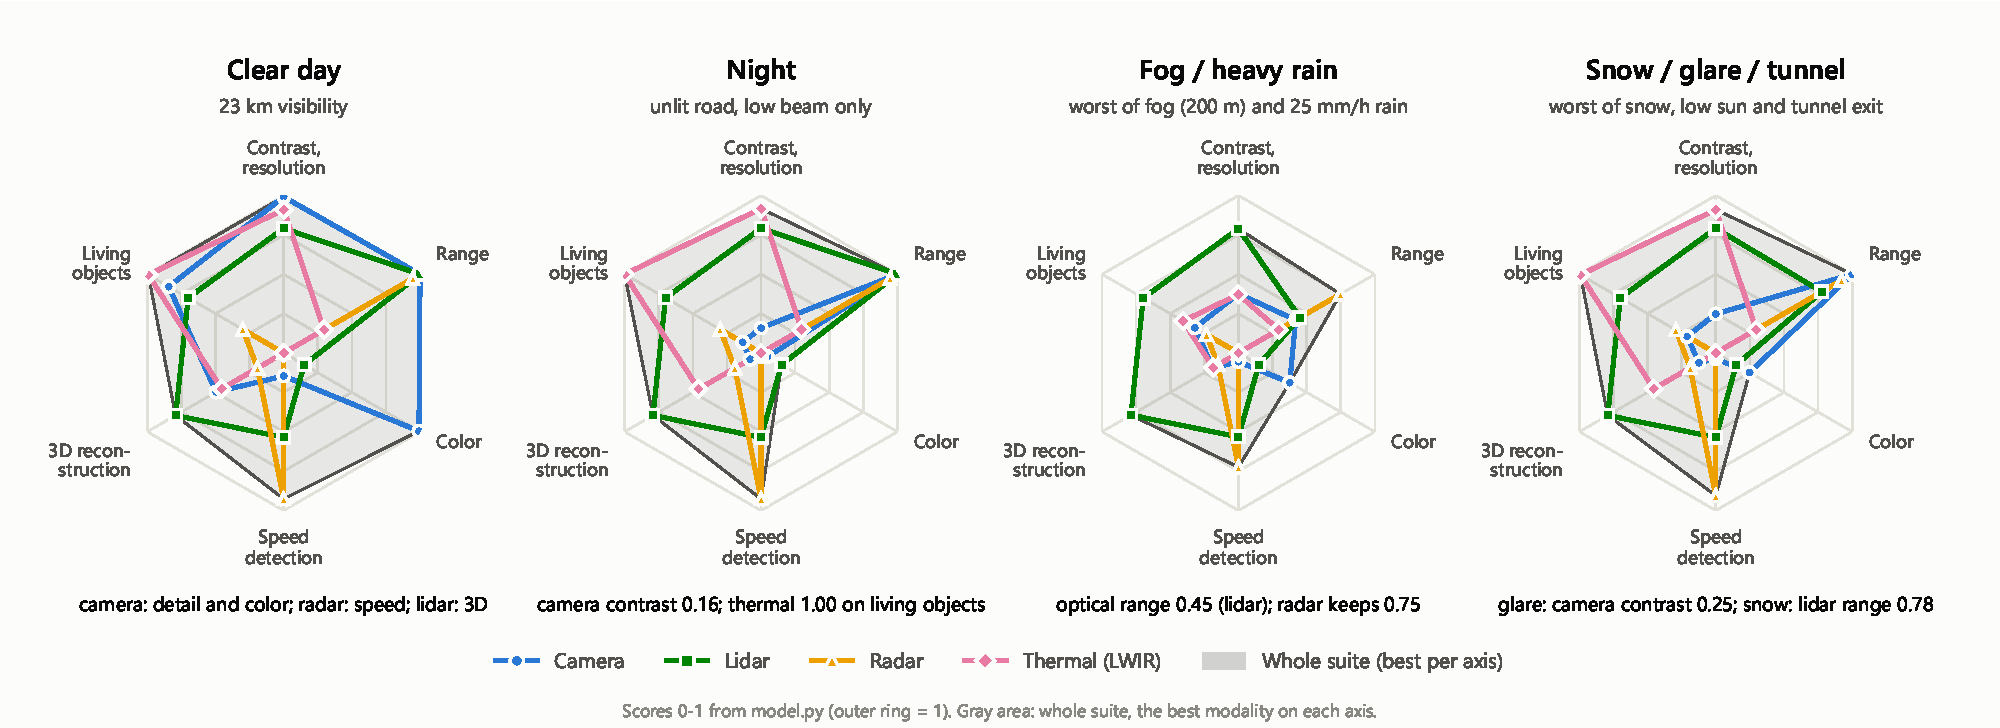
\includegraphics[width=\textwidth]{spider_conditions.pdf}

  \vspace{-0.2em}
  \small
  \begin{columns}[t]
    \column{0.32\textwidth}
    \textbf{Camera}: detail and color, but 0.16 contrast at night, range 0.42 in fog
    \column{0.32\textwidth}
    \textbf{Radar}: speed (0.07\,m/s Doppler) and range in fog; no detail
    \column{0.32\textwidth}
    \textbf{Lidar}: 3D, steady day and night. \textbf{Thermal}: living objects at night
  \end{columns}

  \vspace{0.3em}
  \smallnote{Scores computed from datasheets + one physics law per effect (model.py), not hand-set. Color and the
  living-object cap are rules and labelled so.}
\end{frame}

% ---------------------------------------------------------------
\begin{frame}{3. Design: 20 sensors, each asked for by a number}
  \begin{columns}[c]
    \column{0.40\textwidth}
    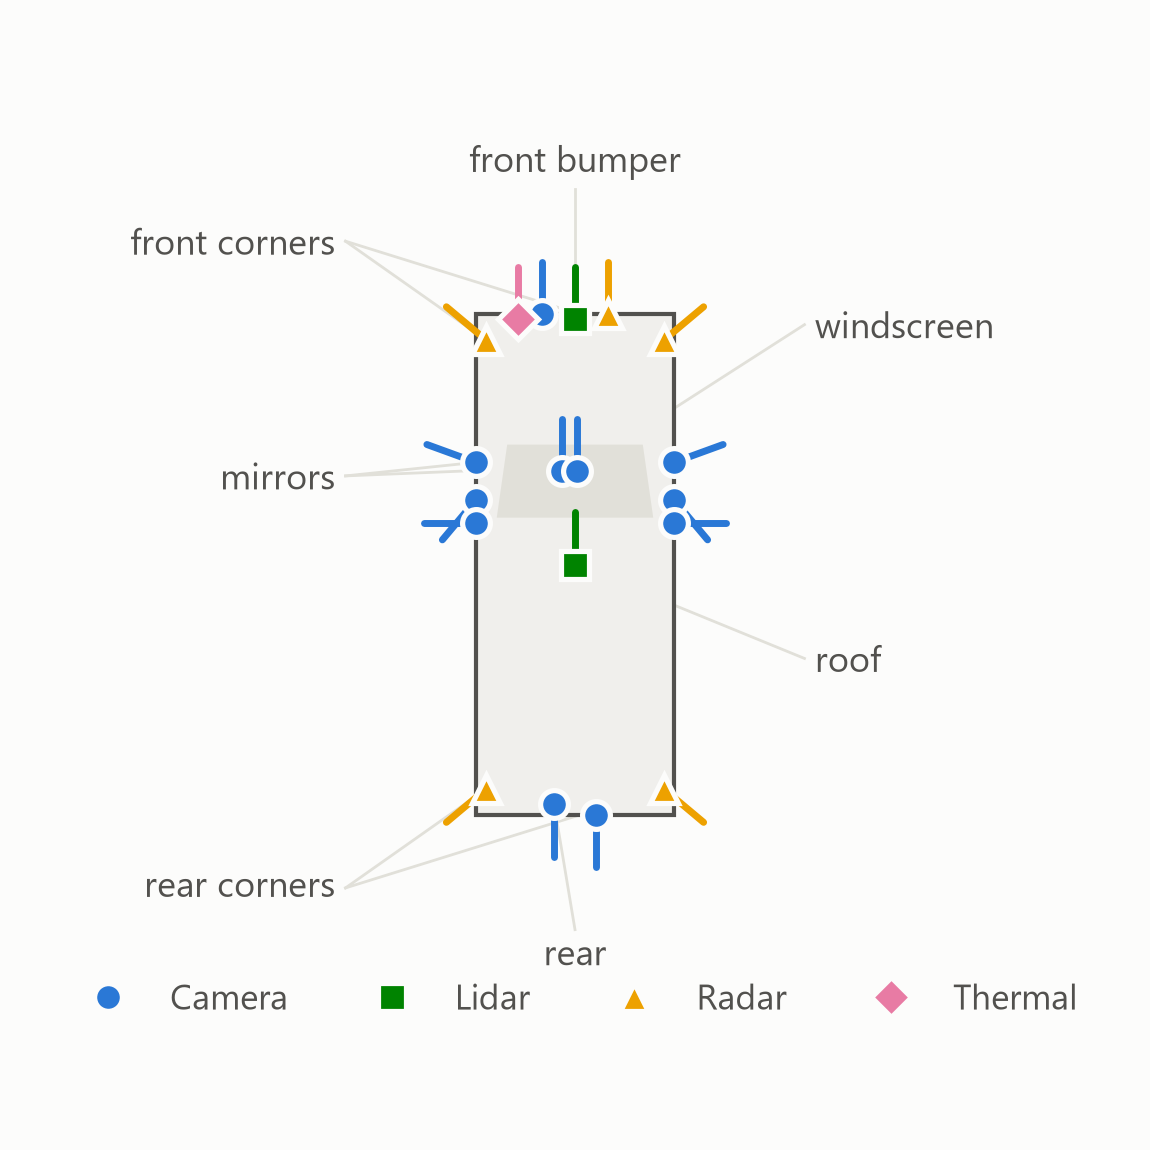
\includegraphics[width=\textwidth]{suite_layout.png}
    \column{0.58\textwidth}
    \scriptsize
    \renewcommand{\arraystretch}{1.12}
    \begin{tabularx}{\textwidth}{@{}rlXr@{}}
      \toprule
      & sensor & why (number from our model) & USD \\
      \midrule
      1 & InnovizTwo lidar, front & dark car at 300\,m, dark pedestrian at 231\,m, day or night & 1,000 \\
      1 & Hesai OT128 lidar, roof & 360$^\circ$ 3D: car at 230\,m $>$ 81\,m sides, 96\,m behind & 3,000 \\
      5 & smartmicro DRVEGRD 171 radar & Doppler 0.07\,m/s; still 239\,m in fog; corners = 2nd modality sideways & 2,000 \\
      3 & 8\,MP OX08B40, 30$^\circ$/60$^\circ$/60$^\circ$ & color, signs, lights; tele sees a car at 464\,m; 140\,dB HDR & 900 \\
      4 & 8\,MP OX08B40, 120$^\circ$, mirrors & cross traffic at the sides: 113\,m $>$ 81\,m & 1,200 \\
      4 & 3\,MP ISX031 fisheye & near field 0.1--5\,m all round & 1,836 \\
      1 & Raytron Horus640-D LWIR & night pedestrians: camera only 63\,m $<$ 82\,m & 800 \\
      1 & u-blox ZED-F9K + HD map & lane-level position ($<$\,0.2\,m RTK) & 250 \\
      \midrule
      \textbf{20} & & \textbf{total (sensors only; most prices estimated)} & \textbf{10,986} \\
      \bottomrule
    \end{tabularx}

    \vspace{0.4em}
    \smallnote{Official datasheets or manufacturer spec pages for every sensor (backup B1).}
  \end{columns}
\end{frame}

% ---------------------------------------------------------------
\begin{frame}{4. Coverage: how many modalities reach the required range?}
  \centering
  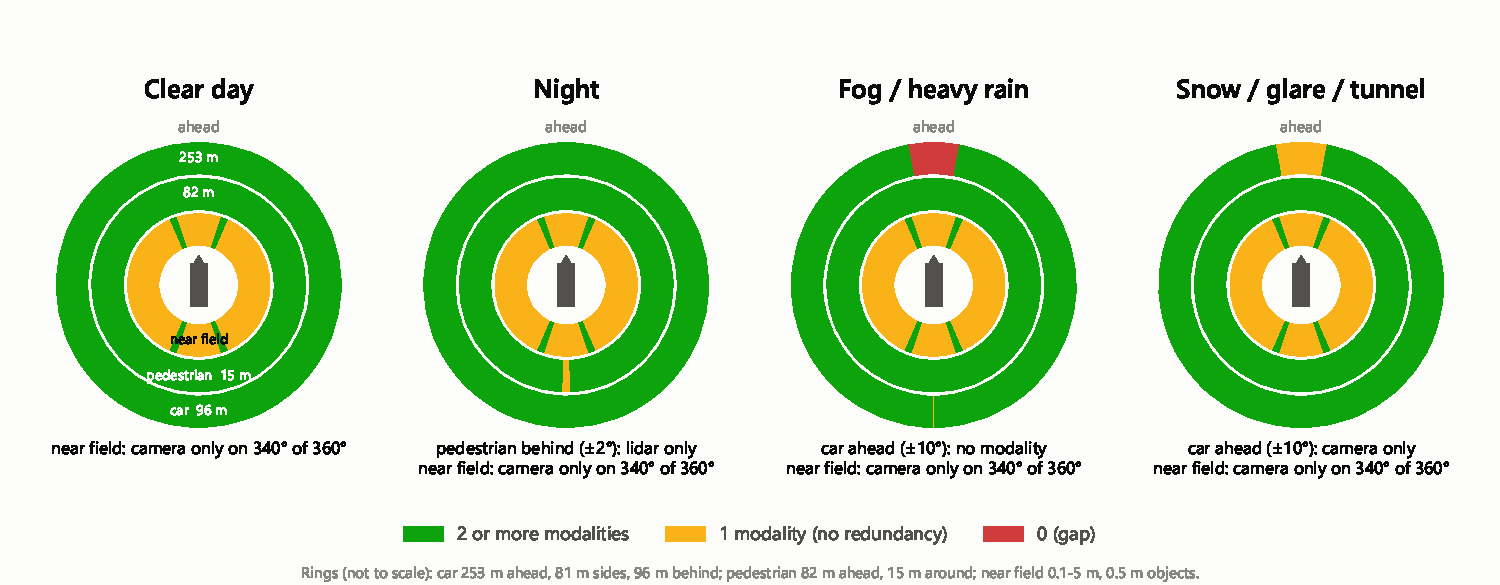
\includegraphics[width=\textwidth]{coverage_conditions.pdf}

  \vspace{-0.3em}
  \small
  \begin{itemize}
    \item Clear day and night: \textcolor{good}{\textbf{2+ modalities on every bearing}} (night: 5$^\circ$ straight behind on lidar only)
    \item Fog: \textcolor{bad}{\textbf{nothing reaches 253\,m ahead}} -- radar 239\,m, lidar 114\,m, camera 106\,m. Snow: camera only
    \item Near field: \textcolor{warn}{\textbf{cameras alone}} -- lidar and radar are blind below 0.2--0.3\,m and beside the doors
  \end{itemize}
\end{frame}

% ---------------------------------------------------------------
\begin{frame}{5. Is Level 5 possible today?}
  \begin{columns}[c]
    \column{0.55\textwidth}
    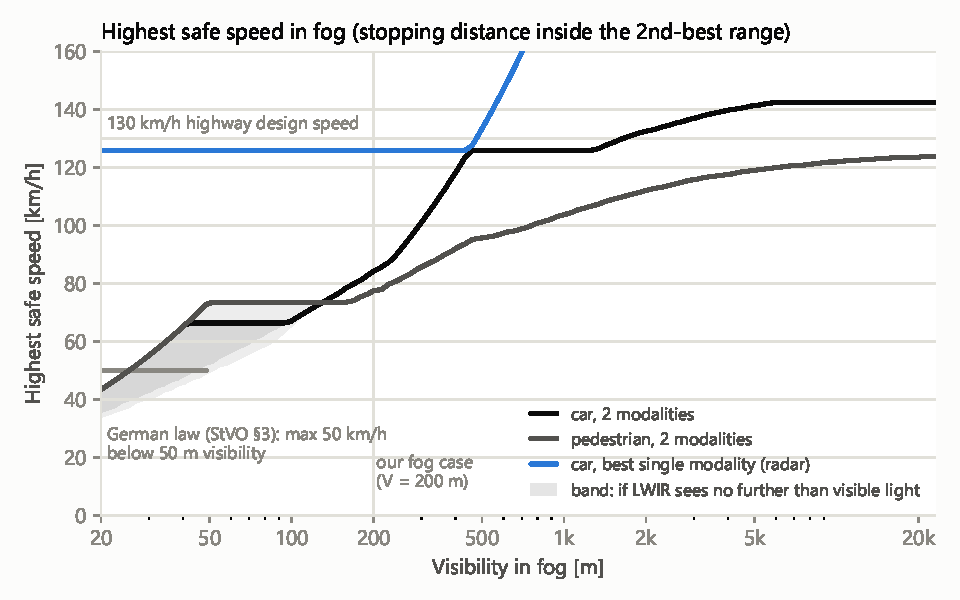
\includegraphics[width=\textwidth]{safe_speed_fog.pdf}

    \vspace{0.2em}
    \scriptsize
    \begin{tabular}{@{}lrr@{}}
      \toprule
      highest speed, 2 modalities over the stopping distance & car & pedestrian \\
      \midrule
      clear day & 142 & 124 \\
      night, unlit road & 142 & \textbf{78} \\
      fog, 200\,m visibility & \textbf{84} & \textbf{77} \\
      snow & 124 & 98 \\
      \bottomrule
    \end{tabular}
    \column{0.43\textwidth}
    \large\textbf{No} -- but \textbf{Level 4} in city + highway, \textbf{yes}.

    \vspace{0.6em}
    \small
    \begin{itemize}
      \item SAE L5 = no operating-domain limit: any road, any weather, no human fallback.
      \item Our maps show where physics stops it: in fog and snow no second modality reaches 253\,m,
        so the car must slow -- to 84\,km/h at 200\,m visibility, 40--70\,km/h below 50\,m.
      \item A blocked sensor (snow, ice, spray) is not in any datasheet: cleaning + safe stop needed.
      \item Beyond sensors: the long tail of rare events (RAND 2016: billions of test miles) and
        regulation that approves only defined domains (UNECE R157, German L4 law 2021).
    \end{itemize}
  \end{columns}
\end{frame}

% ---------------------------------------------------------------
\begin{frame}{6. Summary}
  \begin{columns}[t]
    \column{0.32\textwidth}
    \centering
    {\Huge\textbf{20}}\\[0.2em]
    sensors, 10,986\,USD\\
    \smallnote{2 lidar, 5 radar, 11 camera, 1 thermal, GNSS/IMU}
    \column{0.32\textwidth}
    \centering
    {\Huge\textbf{360$^\circ$}}\\[0.2em]
    2+ modalities at car and pedestrian range, clear day and night
    \column{0.32\textwidth}
    \centering
    {\Huge\textbf{84\,km/h}}\\[0.2em]
    top speed in 200\,m fog: nothing confirms radar at 253\,m
  \end{columns}

  \vspace{1.6em}
  \begin{itemize}
    \item \textbf{Compare:} each modality has a blind axis -- the spider charts come from one physics model.
    \item \textbf{Design:} every sensor is there because a required range asks for it.
    \item \textbf{Verdict:} L4 in city + highway inside a speed envelope; true L5 is not possible today.
    \item \textbf{Next gaps to close:} ultrasonic ring (near field), rear LWIR (night, behind),
      longer-range imaging radar (fog ahead).
  \end{itemize}
\end{frame}

\end{document}
